\documentclass[a4paper, 12pt]{article}%тип документа

%отступы
\usepackage[left=2cm,right=2cm,top=2cm,bottom=3cm,bindingoffset=0cm]{geometry}

%Русский язык
\usepackage[T2A]{fontenc} %кодировка
\usepackage[utf8]{inputenc} %кодировка исходного кода
\usepackage[english,russian]{babel} %локализация и переносы

%Вставка картинок
\usepackage{graphicx}
\graphicspath{{pictures/}}
\DeclareGraphicsExtensions{.pdf,.png,.jpg}

%Графики
\usepackage{multirow}
\usepackage{pgfplots}
\pgfplotsset{compat=1.9}

%Математика
\usepackage{amsmath, amsfonts, amssymb, amsthm, mathtools}

%Заголовок
\author{Валеев Рауф Раушанович \\
группа 825}
\title{\textbf{Работа 2.1.6 \\ 
Эффект Джоуля-Томсона}}

\begin{document}
\maketitle

\newpage
	\textbf{Цель работы:} 1) определение изменения температуры углекислого газа при протекании через малопроницаемую перегородку при разных начальных значениях давления и температуры; 2) вычисление по результатам опытов коэффициентов Ван-дер-Ваалься "а" и "b".

	\textbf{В работе используются:} трубка с пористой перегородкой; труба Дьюара; термостат; термометры; дифференциальная термопара; мокровольтметр; балластный баллон; манометр.

\textbf{Краткая теоретическая справка}

	Эффектом Джоуля-Томсона называется изменение температуры газа, медленно протекающего из области высокого в область низкого давления в условиях хорошей тепловой изоляции.
	
	В работе исследуется изменение температуры идеального газа при его течении по трубке с пористой перегородкой (рис.1). 
	
	Рассматривая 2 произвольных сечения записываем уравнение 
	\[A_1 - A_2 = \left( U_2 + \dfrac{\mu v_2^2}{2} \right) - \left( U_1 + \dfrac{\mu v_1^2}{2} \right) \]
	Учитывая некоторые формулы мы получаем, что 
	\[\mu_{D-T} = \dfrac{\Delta T}{\Delta P} \approx \dfrac{\dfrac{2a}{RT} - b}{C_p} \]
	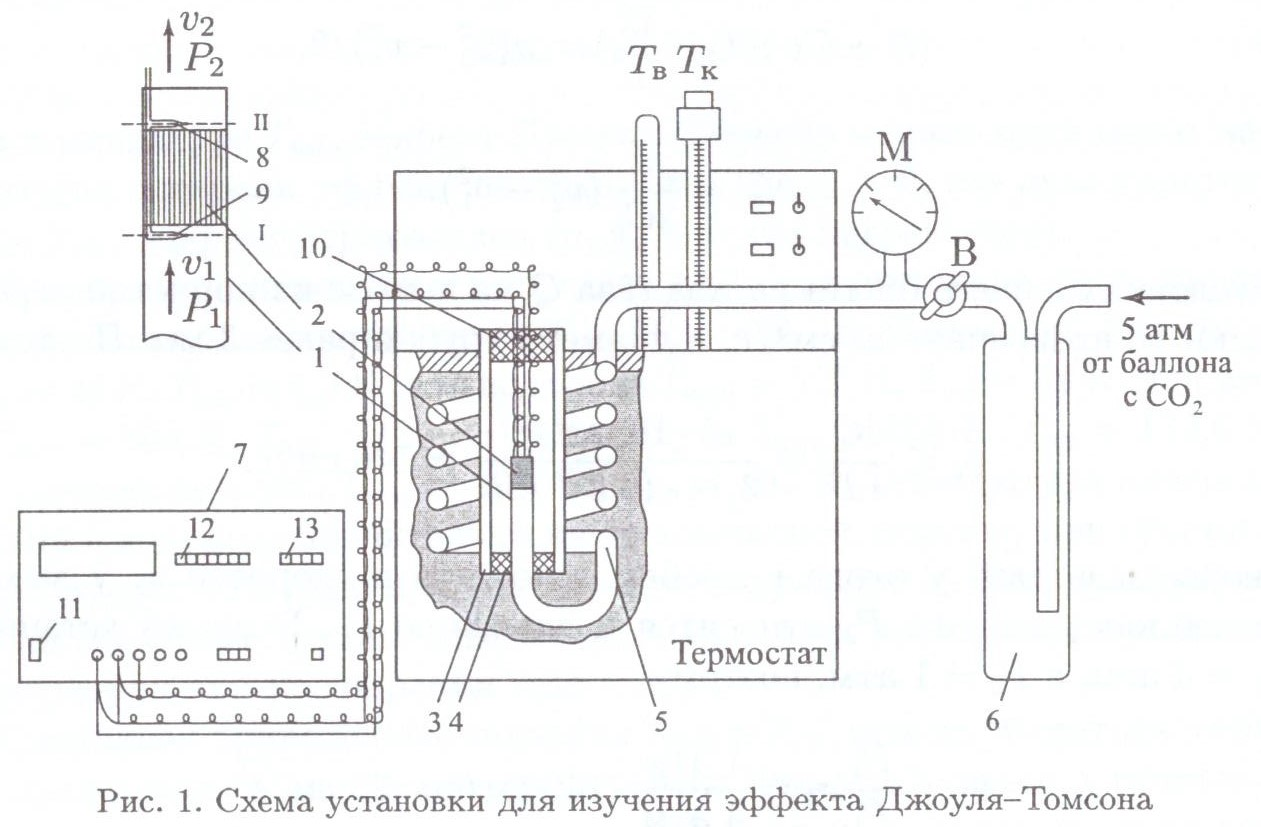
\includegraphics[width = 0.9\textwidth]{216_1.jpg}
	
	\newpage
	
	\textbf{Ход работы}
	\begin{enumerate}
	\item Устанавливаем на контактном термометре температуру, близкую к $T_k$, то есть к комнатной.
	\item Включаем вольтметр и убеждаемся, что изначально он показывает 0. 
	\item Открываем регулирующий вентиль В настолько, чтобы изыбточное давление составило примерно 4 атм.
	\item Через 10-15 минут после подачи давления, когда полностью затухнут переходные процессы, зписываем показания вольтметра. 
	\item Постепенно уменьшаем давления по 0,5 атм и записываем значения вольтметра.
	\item Окончив измерения устанавливаем на термометре температуру в 46 градусов и проводим опять пункты 1-5 для 46 и затем для 70 градусов. Все значения записываем в таблицы.
	\begin{center}
\begin{tabular}{|c|c|c|}
\hline
\multicolumn{3}{|c|}{294 $K$}                             \\ \hline
$\Delta P$, атм & $\Delta U$, мкВ & $\Delta T$, $^{0}K$ \\ \hline
0               & 0,000           & 0,000               \\ \hline
1,3             & 44,000          & 1,081               \\ \hline
1,8             & 63,000          & 1,548               \\ \hline
2,4             & 87,000          & 2,138               \\ \hline
2,7             & 101,000         & 2,482               \\ \hline
3,0             & 112,000         & 2,752               \\ \hline
3,4             & 131,000         & 3,219               \\ \hline
3,7             & 145,000         & 3,563               \\ \hline
4,0             & 160,000         & 3,931               \\ \hline
\end{tabular}
\begin{tabular}{|c|c|c|}
\hline
\multicolumn{3}{|c|}{328 $K$}                         \\ \hline
$\Delta P$, атм & $\Delta U$, мкВ & $\Delta T$, $^0K$ \\ \hline
0,0             & 0,000           & 0,000             \\ \hline
1,0             & 25,000          & 0,588             \\ \hline
1,5             & 38,000          & 0,894             \\ \hline
2,0             & 50,000          & 1,176             \\ \hline
2,5             & 63,000          & 1,482             \\ \hline
3,0             & 85,000          & 2,000             \\ \hline
3,5             & 102,000         & 2,400             \\ \hline
4,0             & 120,000         & 2,824             \\ \hline
\end{tabular}
\begin{tabular}{|c|c|c|}
\hline
\multicolumn{3}{|c|}{348 $K$}                           \\ \hline
$\Delta P$, атм & $\Delta U$, мкВ & $\Delta T$, $^{0}K$ \\ \hline
0,000           & 0,000           & 0,000               \\ \hline
1,000           & 13,000          & 0,295               \\ \hline
1,500           & 19,000          & 0,431               \\ \hline
2,000           & 28,000          & 0,635               \\ \hline
2,500           & 39,000          & 0,884               \\ \hline
3,000           & 48,000          & 1,088               \\ \hline
3,500           & 61,000          & 1,383               \\ \hline
4,000           & 77,000          & 1,746               \\ \hline
\end{tabular}
\end{center}
\newpage
\item Откладываем полученные значения на графике и определяем $\mu_{D-T}$ для каждой температуры.\\
	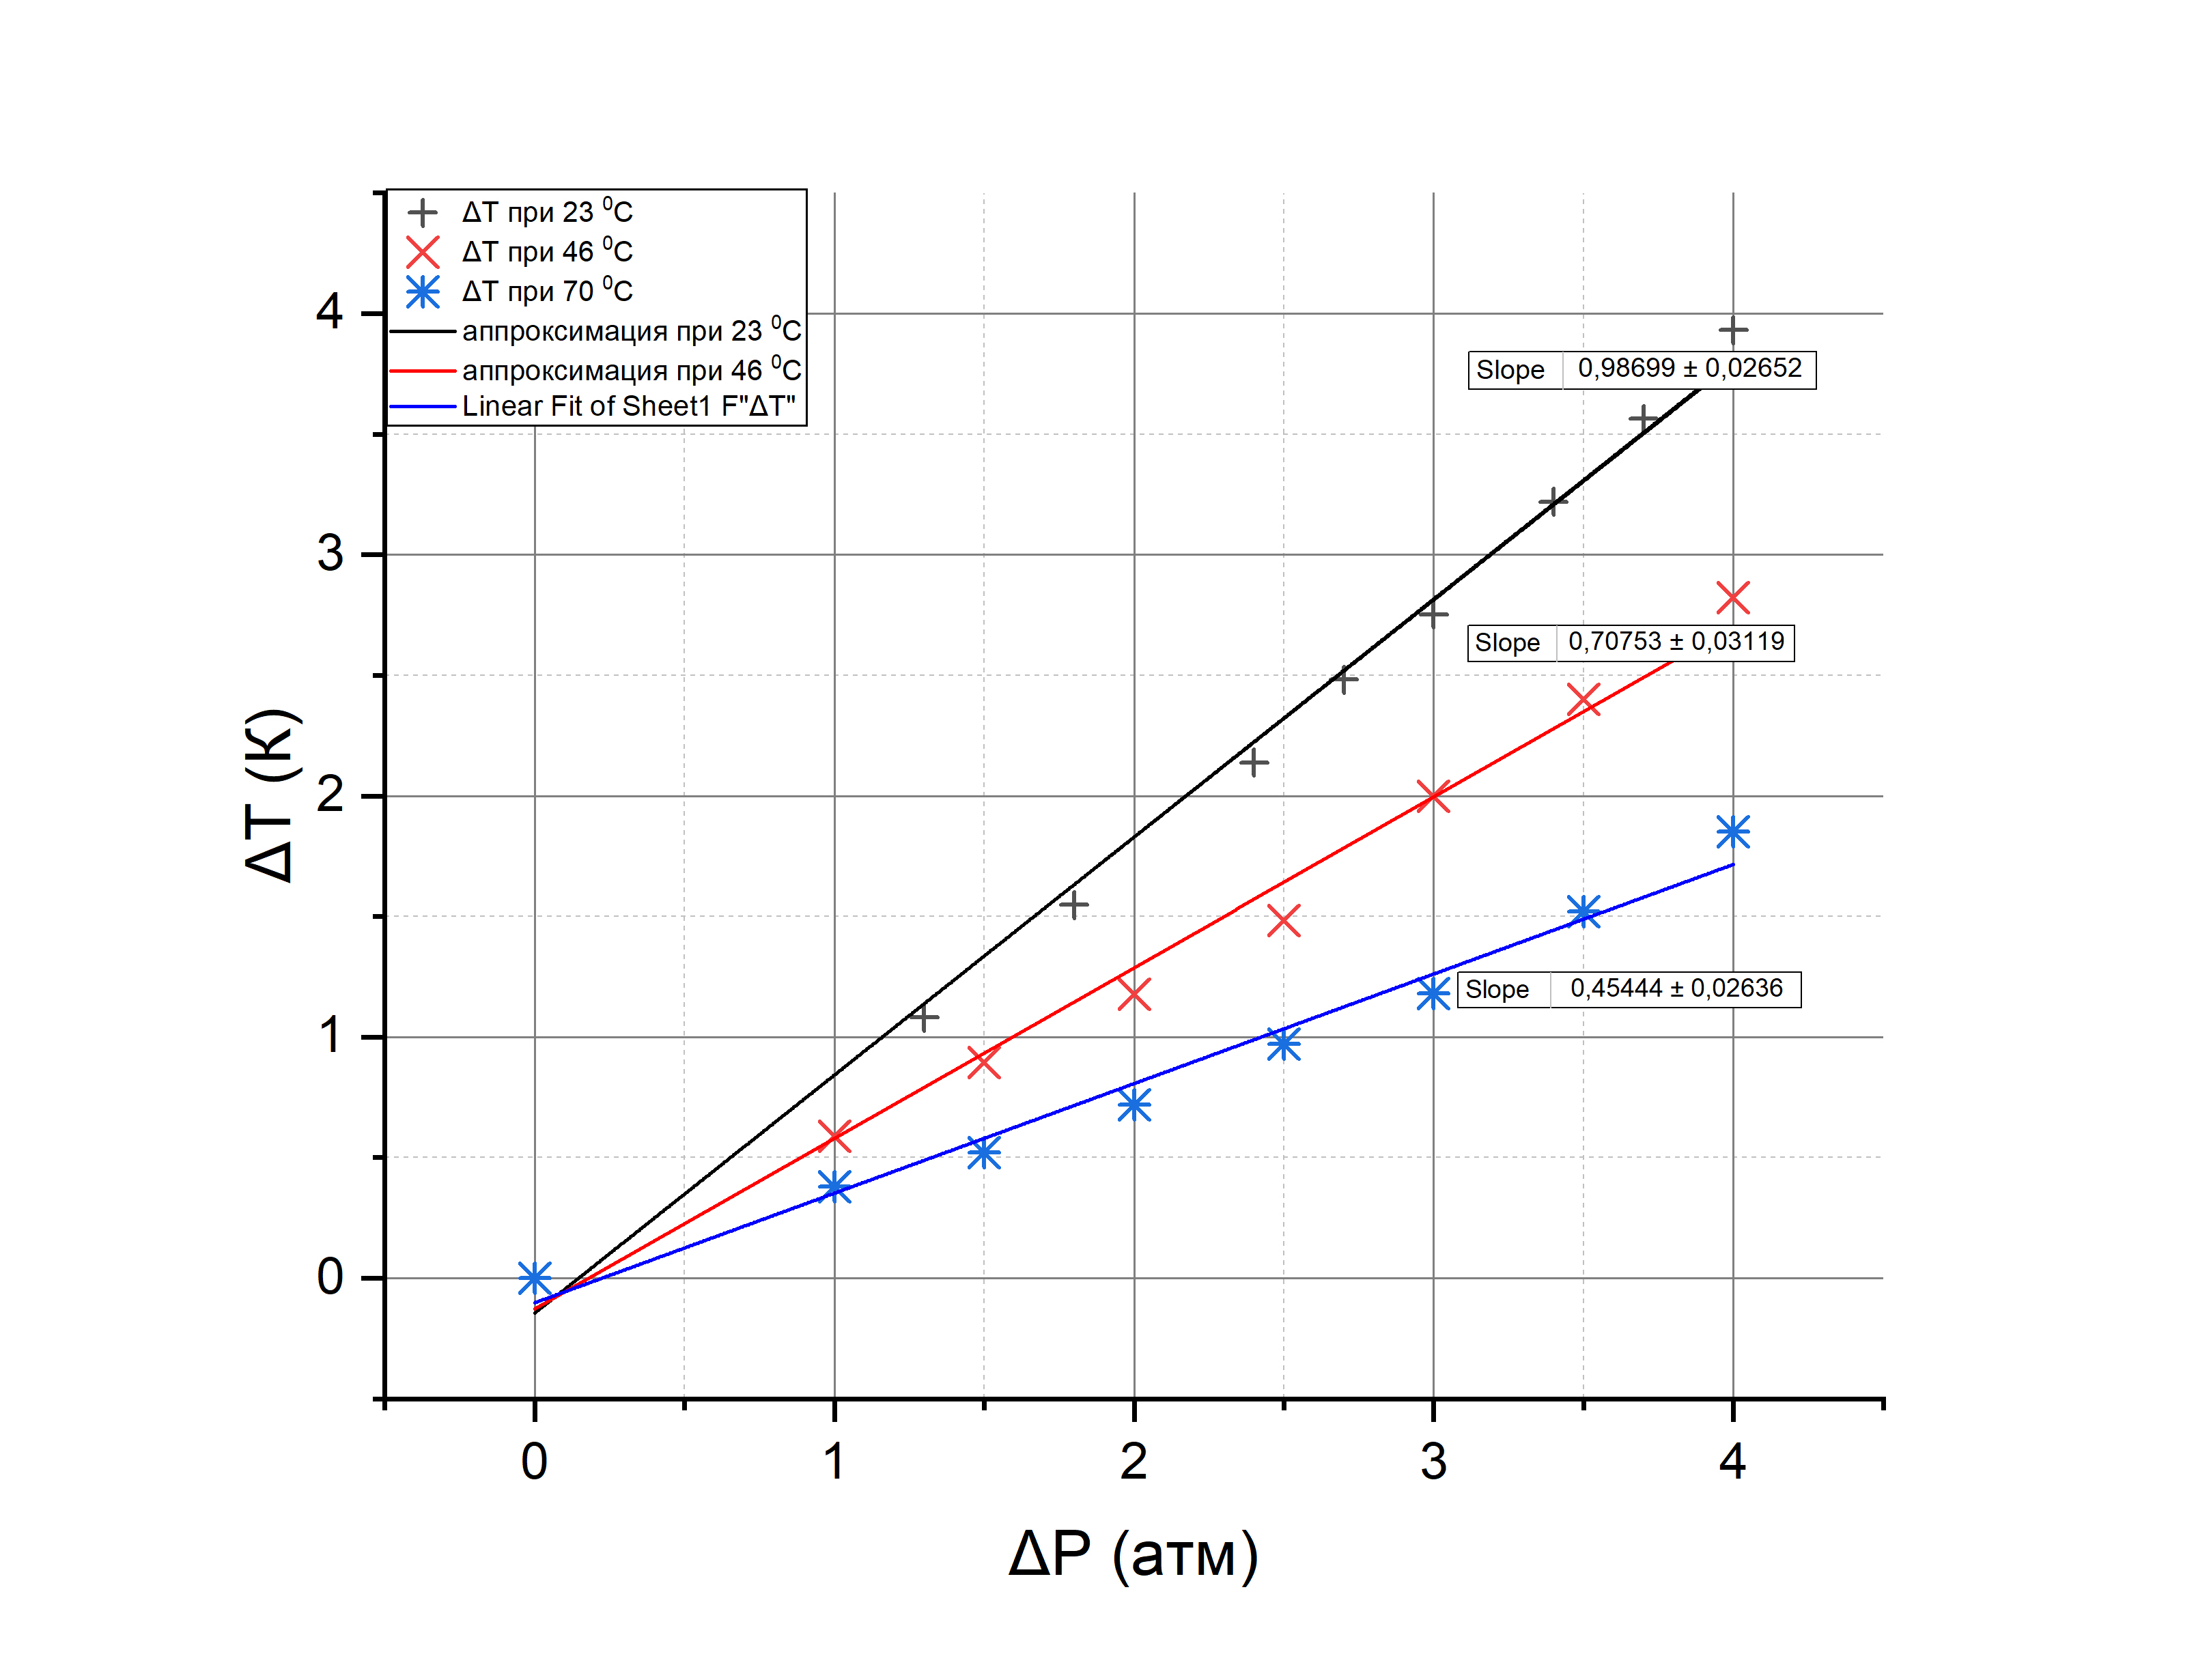
\includegraphics[width = 0.9\textwidth]{216_2.jpg}
	\item решаем систему уравнений:
	\begin{equation*} 
 		\begin{cases}
   			\mu_1 = \dfrac{\dfrac{2a}{RT_1} - b}{4R}\\
   			\\
   			\mu_2 = \dfrac{\dfrac{2a}{RT_2} - b}{4R}\\
   			\\
   			\mu_3 = \dfrac{\dfrac{2a}{RT_3} - b}{4R} 
   			\end{cases}
	\end{equation*}
	из этой системы получаем, что 
	\[a = \dfrac{2R^2(\mu_2 - \mu_1)}{\dfrac{1}{T_1} - \dfrac{1}{T_2}} \]
	\[b = \dfrac{2a}{RT_1} - 4R \mu_1 \]
	\newpage
	\item Все коэффициенты и погрешности для них заносим в таблицу:
	\begin{center}
	\begin{tabular}{|c|c|c|c|}
\hline
$T$, $^0K$ & $\mu$, $^0K$/атм & $\sigma_{\mu}$, $^0K$/атм & $\varepsilon_{\mu}$\\ \hline
294,000    & 0,987            & 0,212                     & 21\%            \\ \hline
328,000    & 0,708            & 0,230                     & 33\%          \\ \hline
348,000    & 0,431            & 0,220                     & 51\%            \\ \hline
\end{tabular}

\begin{tabular}{|c|c|c|c|c|c|c|}
\hline
$a$, $H \cdot m^4 / \text{моль}^4$ & $\sigma_a$, $H \cdot m^4 / \text{моль}^4$ & $\varepsilon_a$ & $b$, $\text{см}^3/\text{моль}$ & $\sigma_b$, $\text{см}^3/\text{моль}$ & $\varepsilon_b$ & $T$, $^0K$\\ \hline
1,095                              & 1,225                                     & 112\%           & 568,046                        & 898,877                               & 158\%   &2309        \\ \hline
\end{tabular}
	\end{center}
	\end{enumerate}
\section*{Уравнение Бертло}
Наблюдаем, что из-за неидеальности системы, а конкретно не изолированности, мы получаем не те значения и огромную погрешность.

Рассмотрим другое приближение идеального газа: по Бертло.
\[\left( p + \dfrac{a}{TV^2} \right) (V - b) = RT\]
\[pV + \dfrac{a}{TV} - \dfrac{ab}{TV^2} - bp = RT\]
\[\left(\dfrac{\partial V}{\partial T} \right)_p \left( p - \dfrac{a}{TV^2} + \dfrac{2ab}{TV^3} \right) - \dfrac{a}{VT^2} + \dfrac{ab}{T^2 V^2} = R\]
\[\left(\dfrac{\partial V}{\partial T} \right)_p = \dfrac{(RV^2T^2 + aV - ab)(V-b)}{T \left( RT^2V^2 - 2a(V-b) + \dfrac{2ab(V-b)}{V} \right)} \Rightarrow \mu = \dfrac{\dfrac{3a}{RT^2} - b}{C_p} \]
Для него получаем:

\begin{equation*} 
 		\begin{cases}
   			\mu_1 = \dfrac{\dfrac{3a}{RT_1^2} - b}{4R}\\
   			\\
   			\mu_2 = \dfrac{\dfrac{2a}{RT_2^2} - b}{4R}\\
   			\\
   			\mu_3 = \dfrac{\dfrac{2a}{RT_3^2} - b}{4R} 
   			\end{cases}
	\end{equation*}
	из этой системы получаем, что 
	\[a = \dfrac{4R^2(\mu_2 - \mu_1)}{3 \left( \dfrac{1}{T_1^2} - \dfrac{1}{T_2^2} \right)} \]
	\[b = \dfrac{3a}{RT_1^2} - 4R \mu_1 \]
	
\begin{tabular}{|c|c|c|c|}
\hline
                                          & Решения системы уравнений & $\sigma$   & $\epsilon$ \\ \hline
$a$, $H \cdot m^4 \cdot K/ \text{моль}^4$ & 113,142            & 126,630 & 111,92\%   \\ \hline
$b$, $\text{см}^3/\text{моль}$            & 144,478                & 533,54 & 369,29\%   \\ \hline
\end{tabular}
\end{document}